% Exercices originaux de remplacement -- chapitres 1 et 2 (séances 1 à 14).
% \DefExo{séance}{cible}{énoncé}{correction détaillée}{nombre de lignes élève}

% -----------------------------------------------------------------------------
% Chapitre 1 -- Suites numériques
% -----------------------------------------------------------------------------
\DefExo{1}{Reconnaître une suite arithmétique par différence}{%
Le responsable d'un entrepôt teste trois modèles. Pour tout entier naturel $n$, $n$ désigne le numéro de la semaine.
\begin{itemize}
\item Nombre de colis préparés : $a_n=3(2n+7)-n$.
\item Nombre de réclamations clients : $b_n=2n^2-n+4$.
\item Nombre de palettes encore en stock : $c_n=150-7n$.
\end{itemize}
\begin{enumerate}[label=\alph*.]
\item Pour chacune des trois suites, calculer $u_{n+1}-u_n$ (avec $u=a$, $b$ ou $c$) et préciser si la suite est arithmétique ; si oui, donner sa raison.
\item Pour chaque suite arithmétique, interpréter la raison dans le contexte.
\end{enumerate}
}{%
\begin{enumerate}[label=\alph*.]
\item \textbf{Suite $(a_n)$.} On développe : $a_n=6n+21-n=5n+21$. Alors $a_{n+1}-a_n=5(n+1)+21-(5n+21)=5$. La différence est constante : $(a_n)$ est arithmétique de raison $5$ (premier terme $a_0=21$).

\textbf{Suite $(b_n)$.} $b_{n+1}-b_n=2(n+1)^2-(n+1)+4-(2n^2-n+4)=2(2n+1)-1=4n+1$. Cette différence dépend de $n$ : par exemple $b_0=4$, $b_1=5$, $b_2=10$, donc $b_1-b_0=1$ et $b_2-b_1=5$. La suite $(b_n)$ n'est pas arithmétique.

\textbf{Suite $(c_n)$.} $c_{n+1}-c_n=150-7(n+1)-(150-7n)=-7$. La suite $(c_n)$ est arithmétique de raison $-7$ (premier terme $c_0=150$).
\item Chaque semaine, l'entrepôt prépare $5$ colis de plus que la semaine précédente. Chaque semaine, le stock diminue de $7$ palettes (raison négative : diminution).
\end{enumerate}
}{4}

\DefExo{2}{Terme général et termes éloignés (arithmétique)}{%
Une entreprise de livraison remplace progressivement ses véhicules diesel par des véhicules électriques. Au début de l'année 2025 (rang $0$), elle possède $186$ véhicules diesel et elle en retire $4$ chaque année. On note $d_n$ le nombre de véhicules diesel au début de l'année $2025+n$ ; la suite $(d_n)$ est arithmétique.
\begin{enumerate}[label=\alph*.]
\item Donner le premier terme $d_0$ et la raison de la suite $(d_n)$.
\item Exprimer $d_n$ en fonction de $n$ pour tout entier naturel $n$.
\item Calculer $d_{12}$ et $d_{30}$. Interpréter $d_{30}$ par une phrase.
\end{enumerate}
}{%
\begin{enumerate}[label=\alph*.]
\item $d_0=186$ ; on retire $4$ véhicules par an, donc $d_{n+1}=d_n-4$ : la raison est $r=-4$.
\item Pour une suite arithmétique de premier terme $d_0$ : $d_n=d_0+nr$, soit $d_n=186-4n$.
\item $d_{12}=186-4\times12=186-48=138$ et $d_{30}=186-4\times30=186-120=66$.

Le rang $30$ correspond à l'année $2025+30=2055$ : selon ce modèle, l'entreprise possèdera encore $66$ véhicules diesel au début de l'année $2055$.
\end{enumerate}
}{4}

\DefExo{3}{Somme de termes consécutifs d'entiers}{%
\begin{enumerate}[label=\alph*.]
\item Calculer $\displaystyle\sum_{i=1}^{365}i=1+2+\cdots+365$.
\item Calculer $\displaystyle\sum_{k=100}^{365}k=100+101+\cdots+365$. Préciser le nombre de termes de cette somme.
\item Pour se constituer une épargne, Lova applique un défi : le $k$-ième jour de l'année, elle dépose $k$ centimes dans une tirelire ($1$ centime le 1\textsuperscript{er} jour, $2$ centimes le 2\textsuperscript{e} jour, etc.). Quelle somme, en euros, aura-t-elle déposée au total sur une année de $365$ jours ? Et entre le 100\textsuperscript{e} et le 365\textsuperscript{e} jour inclus ?
\end{enumerate}
}{%
\begin{enumerate}[label=\alph*.]
\item Les entiers de $1$ à $365$ forment une suite arithmétique de raison $1$ ; il y a $365$ termes. Donc
$\displaystyle\sum_{i=1}^{365}i=365\times\frac{1+365}{2}=365\times183=66\,795$.
\item De $100$ à $365$, il y a $365-100+1=266$ termes. Donc
$\displaystyle\sum_{k=100}^{365}k=266\times\frac{100+365}{2}=266\times232{,}5=61\,845$.

Contrôle : $66\,795-61\,845=4\,950=\dfrac{99\times100}{2}$, qui est bien la somme des entiers de $1$ à $99$.
\item Le total déposé sur l'année est $66\,795$ centimes, soit $667{,}95$~€. Entre le 100\textsuperscript{e} et le 365\textsuperscript{e} jour, Lova dépose $61\,845$ centimes, soit $618{,}45$~€.
\end{enumerate}
}{5}

\DefExo{4}{Terme général d'une suite géométrique}{%
Une application est testée avant son lancement. La semaine $0$, $3$ testeurs l'installent. On suppose que, chaque semaine, le nombre de nouveaux testeurs est multiplié par $4$. On note $v_n$ le nombre de nouveaux testeurs de la semaine $n$ ; la suite $(v_n)$ est géométrique.
\begin{enumerate}[label=\alph*.]
\item Donner le premier terme et la raison de la suite $(v_n)$, puis exprimer $v_n$ en fonction de $n$.
\item Calculer $v_5$ et $v_9$.
\item Le modèle vous semble-t-il réaliste sur une longue durée ? Justifier par une phrase.
\end{enumerate}
}{%
\begin{enumerate}[label=\alph*.]
\item $v_0=3$ et $v_{n+1}=4v_n$ : la raison est $q=4$. Pour une suite géométrique, $v_n=v_0q^n$, donc $v_n=3\times4^n$.
\item $v_5=3\times4^5=3\times1\,024=3\,072$ et $v_9=3\times4^9=3\times262\,144=786\,432$.
\item Non : selon le modèle, il y aurait $786\,432$ nouveaux testeurs la semaine $9$, et plus de $3$ millions la semaine suivante ($v_{10}=3\,145\,728$). Une croissance aussi rapide ne peut pas durer : le nombre d'utilisateurs potentiels est limité.
\end{enumerate}
}{4}

\DefExo{5}{Terme général et somme géométrique}{%
Une association de reboisement plante $1\,500$ arbres la première année de son programme. Grâce à de nouveaux bénévoles, le nombre d'arbres plantés double chaque année. On note $u_0=1\,500$ le nombre d'arbres plantés la première année et $u_n$ le nombre d'arbres plantés la $(n+1)$-ième année.
\begin{enumerate}[label=\alph*.]
\item Justifier que $(u_n)$ est une suite géométrique. Exprimer $u_n$ en fonction de $n$ et en déduire $u_6$.
\item Calculer $S=u_0+u_1+\cdots+u_6$ et interpréter ce résultat dans le contexte.
\end{enumerate}
}{%
\begin{enumerate}[label=\alph*.]
\item Doubler revient à multiplier par $2$ : $u_{n+1}=2u_n$. La suite $(u_n)$ est géométrique de premier terme $u_0=1\,500$ et de raison $q=2$. Donc $u_n=1\,500\times2^n$ et $u_6=1\,500\times2^6=1\,500\times64=96\,000$.
\item La somme comporte $7$ termes (de $u_0$ à $u_6$) et $q\neq1$ :
\[
S=u_0\,\frac{1-q^{7}}{1-q}=1\,500\times\frac{1-2^7}{1-2}=1\,500\times\frac{-127}{-1}=190\,500.
\]
Sur les sept premières années du programme, l'association a planté $190\,500$ arbres au total.
\end{enumerate}
}{5}

\DefExo{6}{Choisir entre modèle arithmétique et géométrique}{%
Pour chaque proposition, dire si elle est vraie ou fausse. Justifier la réponse.
\begin{enumerate}
\item Le prix d'un abonnement annuel de transport augmente de $1{,}50$~€ chaque année. Cette situation peut être modélisée par une suite arithmétique de raison $1{,}5$.
\item Une voiture perd $15\,\%$ de sa valeur chaque année. Cette situation peut être modélisée par une suite géométrique de raison $1{,}15$.
\item Une somme est placée sur un livret à intérêts composés au taux annuel de $3\,\%$, sans aucun dépôt ni retrait. Le capital peut être modélisé par une suite géométrique de raison $1{,}03$.
\item Une cuve de récupération d'eau de pluie contient $1\,000$~L. Chaque jour, elle perd $5\,\%$ de son contenu, puis on y ajoute $40$~L. Le volume peut être modélisé par une suite géométrique de raison $0{,}95$.
\item La population d'une commune augmente de $2\,\%$ par an. Cette situation peut être modélisée par une suite arithmétique de raison $2$.
\item Un prêt de $2\,000$~€ est accordé à intérêts simples au taux annuel de $6\,\%$. La somme due peut être modélisée par une suite arithmétique de raison $120$.
\item Le nombre de visites mensuelles d'un site internet diminue de $300$ chaque mois. Cette situation peut être modélisée par une suite géométrique.
\end{enumerate}
}{%
\begin{enumerate}
\item \textbf{Vrai.} On ajoute $1{,}50$~€ chaque année : $u_{n+1}=u_n+1{,}5$, la variation absolue est constante.
\item \textbf{Faux.} Une baisse de $15\,\%$ correspond au coefficient $1-\dfrac{15}{100}=0{,}85$ : la suite est géométrique de raison $0{,}85$, et non $1{,}15$ (qui traduirait une hausse).
\item \textbf{Vrai.} Chaque année le capital est multiplié par $1+\dfrac{3}{100}=1{,}03$ : $C_{n+1}=1{,}03\,C_n$.
\item \textbf{Faux.} On a $V_{n+1}=0{,}95\,V_n+40$ : une opération additive s'ajoute à la multiplication. Avec $V_0=1\,000$ : $V_1=990$ et $V_2=980{,}5$ ; $\dfrac{V_1}{V_0}=0{,}99$ et $\dfrac{V_2}{V_1}\approx0{,}9904$ ne sont pas égaux, la suite n'est pas géométrique (elle n'est pas non plus arithmétique : $-10\neq-9{,}5$).
\item \textbf{Faux.} Une hausse de $2\,\%$ par an est une évolution relative constante : la suite est géométrique de raison $1{,}02$.
\item \textbf{Vrai.} Aux intérêts simples, les intérêts sont calculés sur la somme initiale : $2\,000\times0{,}06=120$~€ s'ajoutent chaque année. La somme due augmente donc de $120$~€ par an.
\item \textbf{Faux.} La diminution est absolue et constante ($-300$ par mois) : la suite est arithmétique de raison $-300$.
\end{enumerate}
}{6}

% -----------------------------------------------------------------------------
% Chapitre 2 -- Fonctions exponentielles
% -----------------------------------------------------------------------------
\DefExo{7}{Prolonger une suite géométrique en fonction}{%
Au 1\textsuperscript{er} janvier 2024, la puissance des panneaux solaires installés dans une région est de $240$ mégawatts (MW). On estime que cette puissance augmente de $12\,\%$ par an. Pour tout entier naturel $n$, on note $u_n$ la puissance installée, en MW, au 1\textsuperscript{er} janvier de l'année $2024+n$ ; on admet que $(u_n)$ est une suite géométrique.
\begin{enumerate}
\item Donner la raison de la suite $(u_n)$ et exprimer $u_n$ en fonction de $n$.
\item On souhaite estimer la puissance installée à des dates quelconques. Proposer l'expression d'une fonction $f$ donnant la puissance installée $x$ années après le 1\textsuperscript{er} janvier 2024, $x$ étant un nombre réel positif.
\item Estimer, à $0{,}1$~MW près, la puissance installée au 1\textsuperscript{er} janvier 2026, au 1\textsuperscript{er} avril 2027 et au 1\textsuperscript{er} juillet 2029. On assimile un trimestre à $0{,}25$ an.
\end{enumerate}
}{%
\begin{enumerate}
\item Une hausse de $12\,\%$ correspond au coefficient $1+\dfrac{12}{100}=1{,}12$. La raison est $q=1{,}12$ et $u_n=240\times1{,}12^n$.
\item On prolonge la suite aux réels positifs : $f(x)=240\times1{,}12^x$ (on a bien $f(n)=u_n$ pour tout entier $n$).
\item \begin{itemize}
\item 1\textsuperscript{er} janvier 2026 : $x=2$ et $f(2)=240\times1{,}12^2=301{,}056\approx301{,}1$~MW.
\item 1\textsuperscript{er} avril 2027 : $3$ ans et un trimestre, soit $x=3{,}25$ ; $f(3{,}25)=240\times1{,}12^{3{,}25}\approx346{,}9$~MW.
\item 1\textsuperscript{er} juillet 2029 : $5$ ans et demi, soit $x=5{,}5$ ; $f(5{,}5)=240\times1{,}12^{5{,}5}\approx447{,}6$~MW.
\end{itemize}
Selon ce modèle, la puissance installée serait d'environ $301{,}1$~MW, $346{,}9$~MW et $447{,}6$~MW à ces trois dates.
\end{enumerate}
}{5}

\DefExo{8}{Propriétés algébriques des puissances}{%
Écrire chacun des nombres suivants sous la forme d'une seule puissance de $3$ :
\[
a=3^{-2}\times3^{6};\qquad b=\left(3^{1{,}5}\right)^4;\qquad
c=27\times9^{-2};\qquad d=\frac{3^8}{9^3}.
\]
}{%
\begin{itemize}
\item $a=3^{-2+6}=3^4$ (règle $a^xa^y=a^{x+y}$).
\item $b=3^{1{,}5\times4}=3^6$ (règle $(a^x)^y=a^{xy}$).
\item $27=3^3$ et $9=3^2$, donc $9^{-2}=\left(3^2\right)^{-2}=3^{-4}$ ; ainsi $c=3^3\times3^{-4}=3^{-1}$.
\item $9^3=\left(3^2\right)^3=3^6$, donc $d=\dfrac{3^8}{3^6}=3^{8-6}=3^2$.
\end{itemize}
On peut contrôler à la calculatrice, par exemple $c=\dfrac{27}{81}=\dfrac13=3^{-1}$ et $d=\dfrac{6\,561}{729}=9=3^2$.
}{3}

\DefExo{9}{Sens de variation de $t\mapsto ka^t$}{%
Déterminer le sens de variation sur $\mathbb{R}$ des fonctions définies par :
\[
f:t\mapsto3{,}5\times0{,}82^t;\qquad
g:t\mapsto-0{,}6\times1{,}15^t;\qquad
h:t\mapsto-4\times0{,}7^t.
\]
}{%
\begin{itemize}
\item $0<0{,}82<1$, donc $t\mapsto0{,}82^t$ est strictement décroissante ; le coefficient $3{,}5$ est positif et conserve le sens de variation : $f$ est strictement décroissante.
\item $1{,}15>1$, donc $t\mapsto1{,}15^t$ est strictement croissante ; le coefficient $-0{,}6$ est négatif et inverse le sens de variation : $g$ est strictement décroissante.
\item $0<0{,}7<1$, donc $t\mapsto0{,}7^t$ est strictement décroissante ; le coefficient $-4$ est négatif et inverse le sens de variation : $h$ est strictement croissante.
\end{itemize}
Contrôle numérique : $h(0)=-4$, $h(1)=-2{,}8$ et $h(2)=-1{,}96$ : les valeurs augmentent.
}{3}

\DefExo{10}{Taux d'évolution annuel moyen}{%
En cinq ans, une usine a réduit sa consommation d'eau de $27\,\%$.
\begin{enumerate}[label=\alph*.]
\item Donner le coefficient multiplicateur global sur les cinq ans.
\item Calculer le taux d'évolution annuel moyen de la consommation d'eau, à $0{,}1\,\%$ près.
\item Vérifier le résultat en appliquant cinq fois ce coefficient moyen arrondi.
\end{enumerate}
}{%
\begin{enumerate}[label=\alph*.]
\item Une baisse de $27\,\%$ correspond au coefficient global $Q=1-\dfrac{27}{100}=0{,}73$.
\item Si $q$ est le coefficient annuel moyen, alors $q^5=0{,}73$, donc $q=0{,}73^{\frac15}\approx0{,}9390$. Le taux annuel moyen est $t=q-1\approx-0{,}061$ : la consommation d'eau a baissé en moyenne d'environ $6{,}1\,\%$ par an.
\item $0{,}939^5\approx0{,}7300$, ce qui correspond bien à une baisse globale d'environ $27\,\%$.
\end{enumerate}
}{4}

\DefExo{11}{Lectures graphiques sur des courbes $a^x$}{%
On a représenté ci-dessous, dans un repère, les fonctions $f$ et $g$ définies sur $\mathbb{R}$ par $f(x)=1{,}8^x$ et $g(x)=0{,}45^x$, ainsi que la droite d'équation $y=3$.
\begin{center}
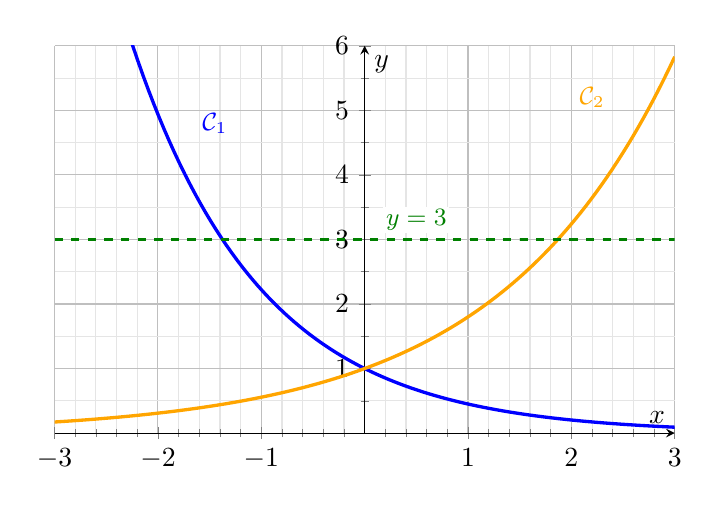
\begin{tikzpicture}
\begin{axis}[width=.78\textwidth,height=6.5cm,axis lines=middle,xmin=-3,xmax=3,ymin=0,ymax=6,
  xtick={-3,...,3},ytick={0,...,6},minor x tick num=4,minor y tick num=1,
  grid=both,major grid style={black!25},minor grid style={black!10},xlabel={$x$},ylabel={$y$}]
\addplot[Blue,very thick,samples=120,domain=-3:3]{0.45^x};
\addplot[Orange,very thick,samples=120,domain=-3:3]{1.8^x};
\addplot[Green,thick,dashed,domain=-3:3]{3};
\node[Blue,font=\small] at (axis cs:-1.45,4.8) {$\mathcal{C}_1$};
\node[Orange,font=\small] at (axis cs:2.2,5.2) {$\mathcal{C}_2$};
\node[Green,font=\small,fill=white,inner sep=1pt] at (axis cs:0.5,3.3) {$y=3$};
\end{axis}
\end{tikzpicture}
\end{center}
\begin{enumerate}
\item Quelle courbe représente la fonction $f$ ? Justifier ce choix.
\item Résoudre graphiquement l'équation $f(x)=3$. À l'aide d'un tableau de valeurs de la calculatrice, donner une valeur approchée de la solution à $0{,}01$ près.
\item Déterminer graphiquement l'ensemble des réels $x$ tels que $f(x)\geqslant3$, puis l'ensemble des réels $x$ tels que $g(x)\geqslant3$.
\end{enumerate}
}{%
\begin{enumerate}
\item $1{,}8>1$, donc $f$ est strictement croissante ; $0<0{,}45<1$, donc $g$ est strictement décroissante. La courbe croissante $\mathcal{C}_2$ représente $f$ (et $\mathcal{C}_1$ représente $g$). Les deux courbes passent par le point $(0;1)$.
\item La courbe $\mathcal{C}_2$ coupe la droite $y=3$ en un point d'abscisse lue proche de $1{,}9$. Avec la calculatrice : $1{,}8^{1{,}86}\approx2{,}984$ et $1{,}8^{1{,}87}\approx3{,}002$, donc la solution est comprise entre $1{,}86$ et $1{,}87$ ; la valeur $1{,}87$ donne l'image la plus proche de $3$. La solution est $x\approx1{,}87$.
\item $f(x)\geqslant3$ lorsque $\mathcal{C}_2$ est au-dessus de la droite $y=3$, c'est-à-dire pour $x\geqslant1{,}87$ environ : $[1{,}87;+\infty[$ (valeur approchée de la borne).

$g$ est décroissante et $\mathcal{C}_1$ coupe la droite $y=3$ pour une abscisse proche de $-1{,}4$ (calculatrice : $0{,}45^{-1{,}38}\approx3{,}010$ et $0{,}45^{-1{,}37}\approx2{,}986$, soit $x\approx-1{,}38$). Ainsi $g(x)\geqslant3$ pour $x\leqslant-1{,}38$ environ : $]-\infty;-1{,}38]$ (valeur approchée de la borne).
\end{enumerate}
}{5}

\DefExo{12}{Inéquations avec une même base}{%
Résoudre sur $\mathbb{R}$ les inéquations suivantes.
\begin{enumerate}[label=\alph*.]
\item $0{,}7^x\leqslant0{,}7^{-1}$
\item $2{,}5^{x+1}>2{,}5^4$
\item $0{,}5^x\geqslant0{,}25$
\end{enumerate}
}{%
\begin{enumerate}[label=\alph*.]
\item $0<0{,}7<1$ : la fonction $x\mapsto0{,}7^x$ est strictement décroissante, elle inverse l'ordre. Donc $0{,}7^x\leqslant0{,}7^{-1}\iff x\geqslant-1$. Ensemble des solutions : $[-1;+\infty[$.
\item $2{,}5>1$ : la fonction $x\mapsto2{,}5^x$ est strictement croissante, elle conserve l'ordre. Donc $2{,}5^{x+1}>2{,}5^4\iff x+1>4\iff x>3$. Ensemble des solutions : $]3;+\infty[$.
\item $0{,}25=0{,}5^2$, donc l'inéquation s'écrit $0{,}5^x\geqslant0{,}5^2$. Comme $x\mapsto0{,}5^x$ est strictement décroissante : $x\leqslant2$. Ensemble des solutions : $]-\infty;2]$.
\end{enumerate}
}{3}

\DefExo{13}{Modéliser par $f(t)=ka^t$ et calculer}{%
Juste après une injection, la concentration d'un médicament dans le sang d'un patient est de $80$~mg/L. Cette concentration diminue ensuite de $15\,\%$ chaque heure. Il s'agit d'une décroissance exponentielle.

On la modélise par une fonction $C$ du temps $t$, exprimé en heures, vérifiant $C(t)=ka^t$.
\begin{enumerate}
\item Déterminer les constantes $k$ et $a$.
\item Calculer la concentration au bout de $3$~h~$30$~min, à $0{,}1$~mg/L près.
\item Le médecin prévoit une nouvelle injection dès que la concentration passe sous $50$~mg/L. Est-ce déjà le cas au bout de $3$~h~$30$~min ? Répondre par une phrase.
\end{enumerate}
}{%
\begin{enumerate}
\item $C(0)=k\times a^0=k$, et $C(0)=80$, donc $k=80$. Une baisse de $15\,\%$ par heure correspond au coefficient $1-\dfrac{15}{100}=0{,}85$, donc $a=0{,}85$ et $C(t)=80\times0{,}85^t$.
\item $3$~h~$30$~min $=3{,}5$~h. $C(3{,}5)=80\times0{,}85^{3{,}5}\approx45{,}3$~mg/L.
\item $45{,}3<50$ : au bout de $3$~h~$30$~min, la concentration est déjà passée sous $50$~mg/L, la nouvelle injection est donc prévue (d'ailleurs $C(3)\approx49{,}1$~mg/L, la concentration est sous ce seuil dès $3$~h).
\end{enumerate}
}{4}

\DefExo{14}{Taux moyen de deux évolutions successives}{%
\begin{enumerate}
\item Le cours d'une monnaie numérique augmente de $125\,\%$ une année, puis baisse de $36\,\%$ l'année suivante. Quel est le taux d'évolution annuel moyen sur ces deux années ?
\item Le prix d'une matière première augmente de $80\,\%$ un mois, puis baisse de $55\,\%$ le mois suivant. Quel est le taux d'évolution mensuel moyen ?
\item Un élève affirme que, dans la question 2, le taux moyen est $\dfrac{80-55}{2}=12{,}5\,\%$. Expliquer par une phrase pourquoi il se trompe.
\end{enumerate}
}{%
\begin{enumerate}
\item Les coefficients sont $1+\dfrac{125}{100}=2{,}25$ et $1-\dfrac{36}{100}=0{,}64$. Le coefficient global est $2{,}25\times0{,}64=1{,}44$. Le coefficient annuel moyen $q$ vérifie $q^2=1{,}44$, donc $q=\sqrt{1{,}44}=1{,}2$ : hausse annuelle moyenne de $20\,\%$.
\item Les coefficients sont $1{,}8$ et $0{,}45$ ; le coefficient global est $1{,}8\times0{,}45=0{,}81$. Le coefficient moyen est $\sqrt{0{,}81}=0{,}9$, soit une baisse mensuelle moyenne de $10\,\%$.
\item Les évolutions successives se composent en multipliant les coefficients, pas en additionnant les taux : la baisse de $55\,\%$ s'applique à un prix déjà augmenté. Sur les deux mois, le prix est multiplié par $0{,}81$ (baisse globale de $19\,\%$), ce qui correspond à une baisse moyenne de $10\,\%$ par mois et non à une hausse de $12{,}5\,\%$.
\end{enumerate}
}{5}
